% @author Arian Helberg

\chapter{Konzepte}
\ldots

\section{Probleme \& Lösungsansätze}
\ldots

\section{Softwarearchitektur}

Die Gliederung der Inhalte für die Softwarearchitektur erfolgt nach der arc42-Vorlage~\cite{arc42}

\subsection{Einführung und Ziele}
Ziel ist die Erstellung eines Programms zur Synthetisierung von Ähnlichkeitsabbildungen einer vom Benutzer
erstellten Verzweigungsstruktur mittels Inferieren und Optimieren von L-Systemen.
Die wesentlichen Features des Programms sind:
\begin{itemize}
    \item Erstellung einer Verzweigungsstruktur über eine grafische Benutzeroberfläche (\textbf{GUI})
    \item Einbindung atomarer Strukturen über externe Dateien
    \item Synthetisierung von ähnlichen Verzweigungsstrukturen anhand der erstellten Struktur
    \item Anzeigen von Verzweigungsstrukturen
\end{itemize}
Priorisierte (absteigend) Qualitätsziele, die bei der Erstellung des Systems umgesetzt werden sollten:
\begin{itemize}
    \item \textbf{Funktionalität} durch Umsetzung aller Teilsysteme
    \item \textbf{Interoperabilität} durch Nutzen einer allgemeinen Repräsentation von L-Systemen, damit diese
    auch in anderen Programmen oder Algorithmen verwendet werden kann
    \item \textbf{Erweiterbarkeit} durch offene Entwurfsmuster (Design Pattern)
    \item \textbf{Modular}e Implementierung für effiziente Wartung und Erweiterung
    \item \textbf{Effizienz} durch effiziente Programmierung
    \item \textbf{Attraktivität} durch intuitive Benutzung (Benutzerfreundlichkeit)
    \item \textbf{Plattformunabhängigkeit} durch Verwenden des Java-Frameworks
\end{itemize}

\subsection{Kontextabgrenzung}
\begin{figure}[H]
    \centering
    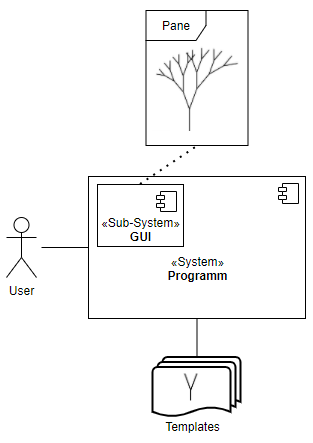
\includegraphics[width=6.2cm]{../images/Fachlicher_Kontext.PNG}
    \caption{System und Systemumgebung}
\end{figure}
\begin{figure}[H]
    \centering
    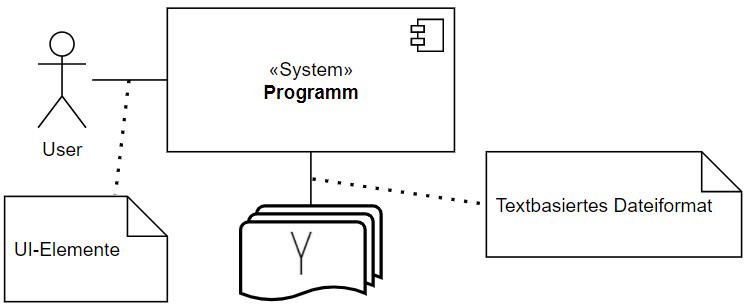
\includegraphics[width=10cm]{../images/Technischer_Kontext.PNG}
    \caption{Technische Interaktion zwischen System und Systemumgebung}
\end{figure}

\newpage

\subsection{Lösungsstrategie}
Gewählte Architekturansätze zur Erreichung der Qualitätsziele:
\begin{center}
    \begin{tabular}{l|l}
        \textbf{Qualitätsziel} & \textbf{Architekturansatz} \\
        \hline \\
        Funktionalität &
        \begin{minipage}[t]{0.8\textwidth}
            \begin{itemize}
                \item Grafische Benutzerschnittstelle: \textit{GUI}
                \item Generieren der Baumstruktur: \textit{TreeGenerator}
                \item Ableiten von L-Systemen aus Baumstrukturen: \textit{Inferer}
                \item Generalisieren von L-Systemen: \textit{Generalizer}
                \item Randomisieren von L-System Parametern: \textit{Randomizer}
            \end{itemize}
        \end{minipage} \\
        \\ \hline \\
        Interoperabilität &
        \begin{minipage}[t]{0.8\textwidth}
            Durch das Nutzen allgemeingültiger mathematischer Beschreibungen sollen erstellte
            L-Systeme in Fremdsystemen, wie Online Visualisierer, genutzt werden können
        \end{minipage} \\
        \\ \hline \\
        Erweiterbarkeit &
        \begin{minipage}[t]{0.8\textwidth}
            Das Nutzen des \textbf{Pipeline Design Pattern}s soll das Erweitern des Systems durch
            Hinzufügen weiterer Teilschritte (\textbf{Pipes}) erleichtern.
            Trennung der grafischen Oberfläche und der Logik durch Aufbauen des Szenengraphen über ein
            XML-Dateiformat
        \end{minipage} \\
        \\ \hline \\
        Modularität &
        \begin{minipage}[t]{0.8\textwidth}
            Sowohl eine sinnvolle Aufteilung von Funktionalitäten auf Dateien und Pakete (\textbf{Package}s), als
            auch effiziente Datenkapselung und geschlossene Informationskontexte sorgen für Modularität des
            Programms
        \end{minipage} \\
        \\ \hline
    \end{tabular}
\end{center}

\subsection{Bausteinsicht}
\underline{Ebene 1}
\begin{figure}[H]
    \centering
    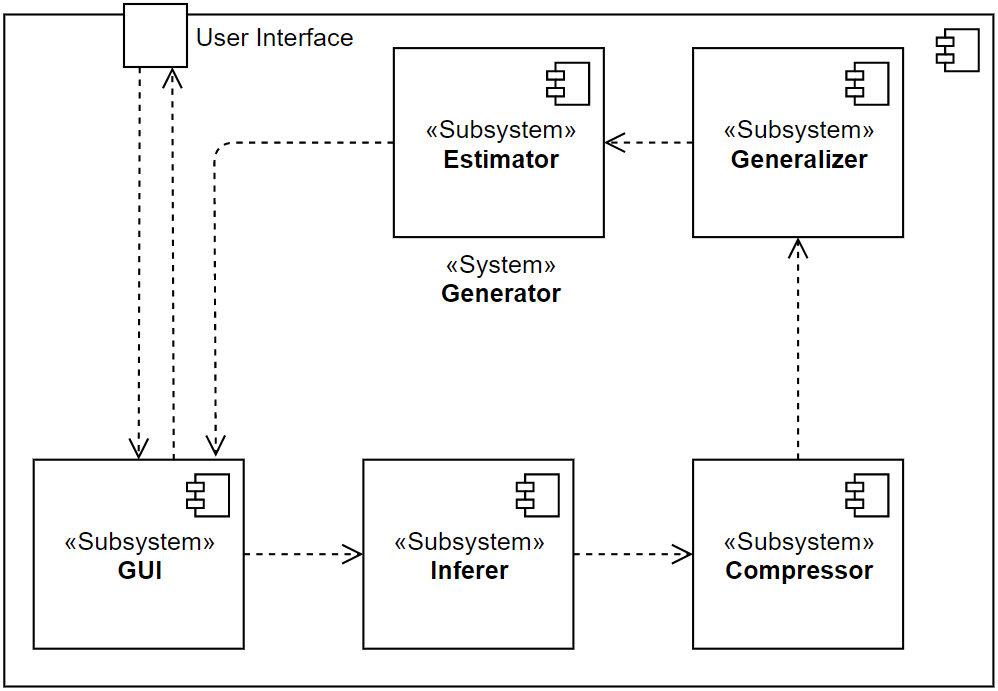
\includegraphics[width=12cm]{../images/Bausteinsicht_Ebene_1.PNG}
    \caption{Subsysteme mit fachlichen Abhängigkeiten}
\end{figure}
\underline{Ebene 2}
\begin{figure}[H]
    \centering
    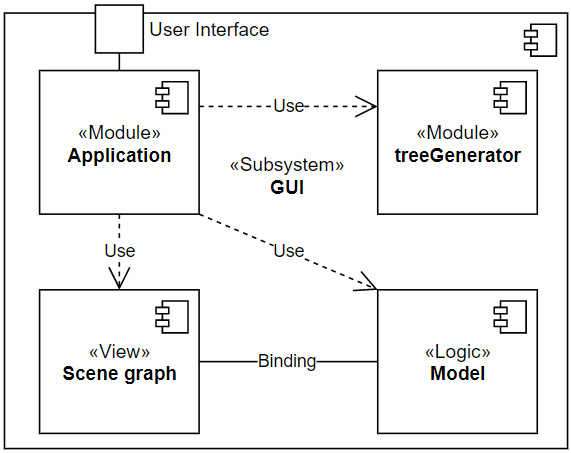
\includegraphics[width=9cm]{../images/Bausteinsicht_Ebene_2.PNG}
    \caption{Subsystem GUI}
\end{figure}

\subsection{Laufzeitsicht}
\begin{figure}[H]
    \centering
    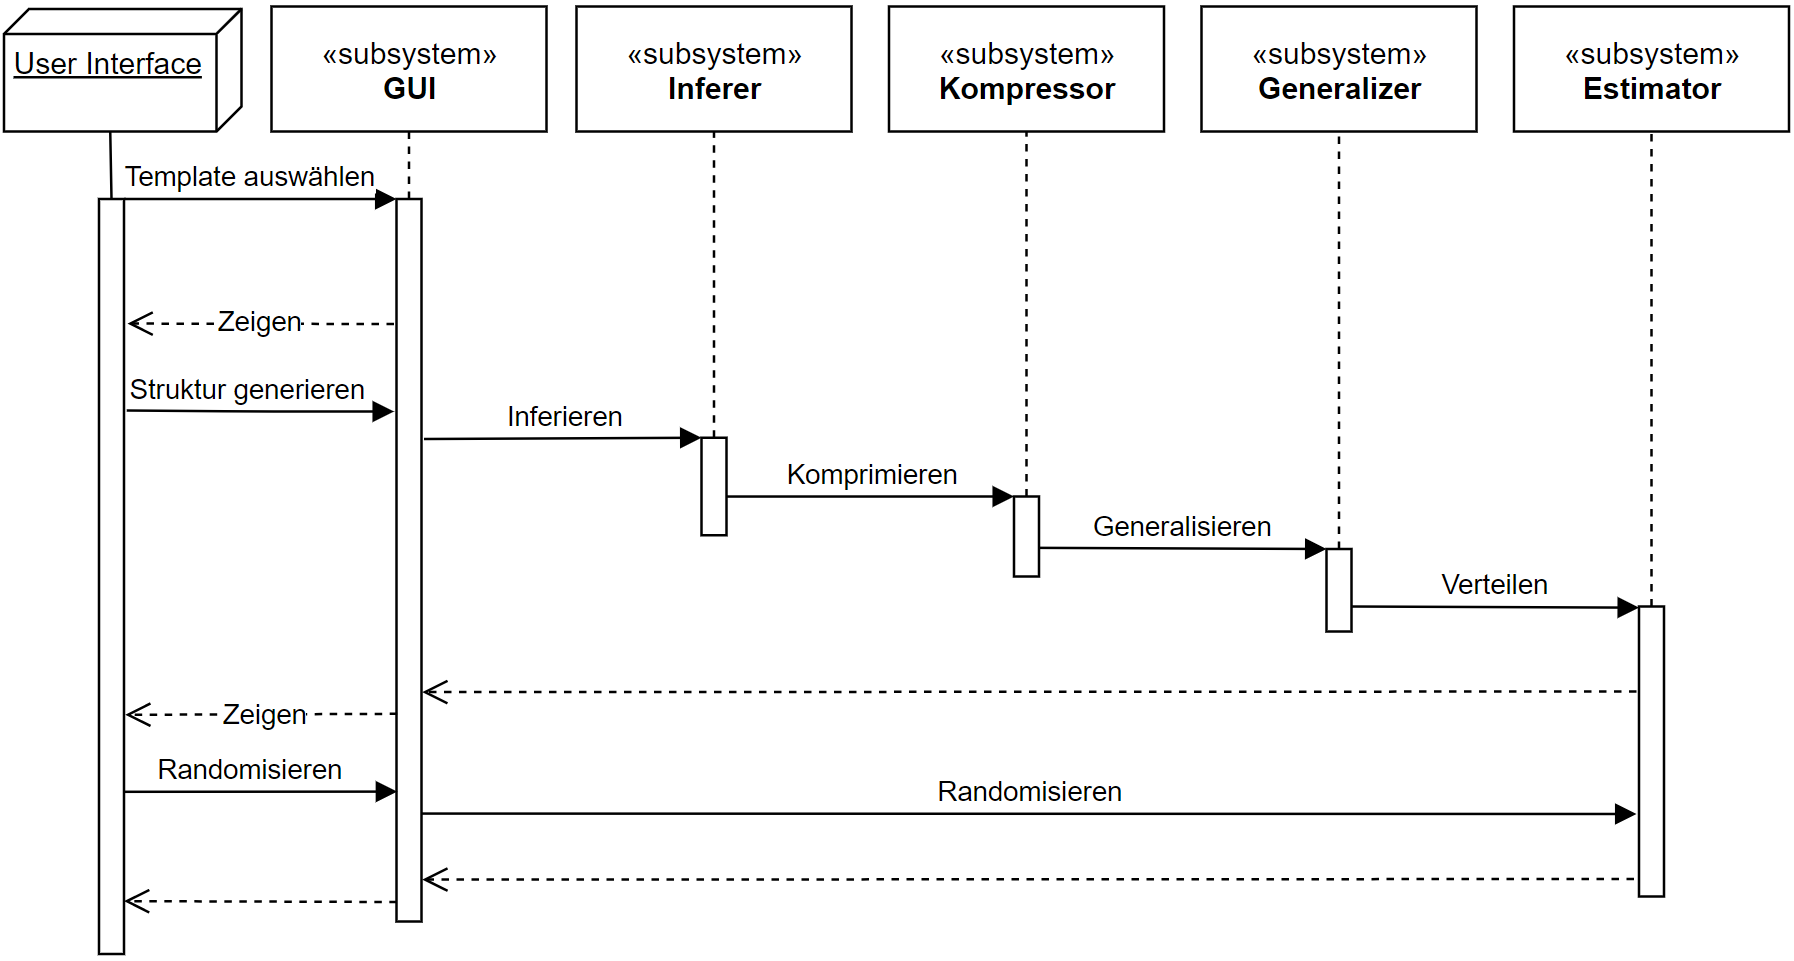
\includegraphics[width=14cm]{../images/Laufzeitsicht.PNG}
    \caption{Laufzeitsicht}
\end{figure}

\subsection{Verteilungsicht}
\begin{figure}[H]
    \centering
    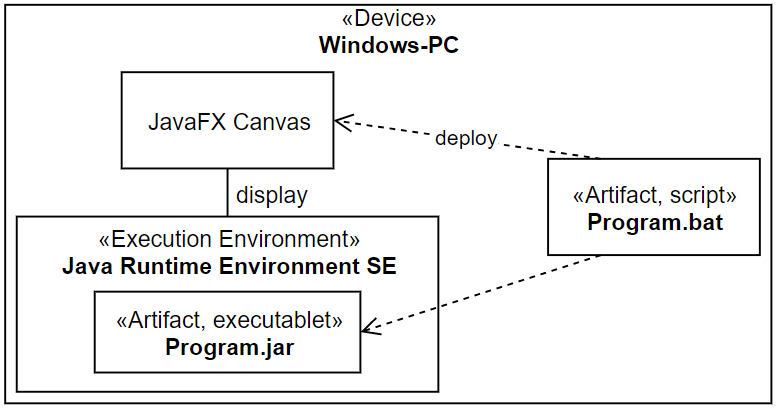
\includegraphics[width=10cm]{../images/Verteilungssicht.PNG}
    \caption{Infrastruktur Windows-PC}
\end{figure}

\subsection{Konzepte}

\subsubsection{Testbarkeit}
Um eine ausreichende Testabdeckung zu erreichen, werden Klassen als kleinstmögliche zu testende Einheit definiert
und durch Komponententests geprüft.
Der Name eines Tests setzt sich aus dem Präfix als Name der zu testenden Klasse oder Releases und dem Suffix
"`Test"'
zusammen.
Testsubjekte werden als \textbf{Blackbox} behandelt, also anhand der Spezifikation getestet.
\begin{center}
    Bsp.: Klasse \textit{Inferer} mit Komponententest \textit{InfererTest}
\end{center}
Da jedes Release der Implementierung ein funktionsfähiges System beinhaltet, kann auf Integrationstests
verzichtet werden.
Weiter wird ein Release anhand von funktionalen und nicht-funktionalen Anforderungen getestet.
Anhand dieser Systemtests wird geprüft, ob Gesamtspezifikationen umgesetzt worden sind.
\begin{center}
    Bsp.: Release 2 mit Systemtest \textit{Release2Test}
\end{center}
Zum Schluss der Implementierung wird ein Akzeptanztest durchgeführt.

\subsubsection{Validierung}
Der Benutzer des Systems nutzt ein grafische Schnittstelle.
Somit kann sichergestellt werden, dass dieser keine ungültigen Eingaben tätigt.
Werden Template-Dateien unter einem bestimmten Dateipfad nicht gefunden, wird eine \textit{NotFound}-Exception
protokolliert und dem Benutzer eine Nachricht über ein Pop-up mitgeteilt.
Eine \textit{IllegalArgumentException} wird verzeichnet und ausgegeben, wenn eingelesene Template-Dateien
strukturelle Fehler aufweisen.

\subsubsection{Fehlerbehandlung}
Zur Fehlersuche und -behandlung biete sich eine Protokollierung über Vorgänge, Fehler und Ausnahmen an.
Bestimmte Fehler werden dem Benutzer weitergegeben und grafisch angezeigt.
Folgende Subsysteme werden in das Programm integriert:
\begin{itemize}
    \item Ausnahmebehandlung (Exception Handling) und
    \item Protokollierung (Logging)
\end{itemize}
Erwartete Exceptions werden jeweils mit eigenen Klassen abgebildet, die von einer entsprechenden Klasse aus der
Exception-Hierarchie abgeleitet sind.
Das Logging ist statisch und überall im System zugreifbar, um eine einheitliche Protokollierung zu gewährleisten.

\subsubsection{Datenstrukturen}
TODO: Klassendiagramm aus IntelliJ generieren

\subsubsection{Workflows \& Algorithmen}
Um als Benutzer des Systems eine Verzweigungsstruktur zu erstellen, wird folgender Arbeitsablauf umgesetzt:
\begin{algorithm}[caption={Erstellen einer Verzweigungsstruktur}, label={alg1}]
    Erster Anker ist vorselektiert
    Wiederhole, bis Struktur fertiggestellt ist:
    Selektiere ein Template aus der Liste
    Setzt Parameter
    Bestätige Auswahl und Parameter
    Zeichne ausgewähltes Template mit Parameternd
    Wähle nächsten Anker aus
\end{algorithm}
\\~\\~\\
Aus der Verzweigungsstruktur kann nun ein L-System erzeugt werden:
\\~\\
Für $\mathcal{L}=\langle M,\omega,R \rangle$:
\begin{algorithm}[caption={Inferieren eines L-Systems aus einer Baumstruktur}, label={alg2}]
    Initialisierung:
    $M=\{F,S\}$
    $\omega=S$
    $R \gets \{\alpha$: $S \rightarrow A\}$
    $\beta=$ nächster Knoten*
    $M \gets \gamma \in \{A,B,\dots,Z\}$, mit $\gamma \notin M$

    Schleife:
    $\delta=$ Wort von $\beta$
    $\forall \{X,Y,Z\} \in \delta:$
    Ersetze mit $\zeta \in \{A,B,\dots,Z\}$, mit $\zeta \notin M$
    $M \gets \zeta$
    $R \gets \{\gamma\rightarrow\delta\}$
    Wenn es ein Symbol $\eta$ in $M\setminus\{F,S\}$ gibt mit $\{\eta \rightarrow bel.\} \notin R$:
    $\gamma=\eta$
    Sonst:
    Breche Schleife ab
    $\beta=$ nächster Knoten*
\end{algorithm}
\blfootnote{* nach Breitensuche, beginnend bei Wurzelknoten S}

\newpage

Um ein kompakteres, gewichtetes L-System zu erzeugen, werden sich wiederholende Unterrbäume gesucht und ersetzt.
Die Gewichtung wird angewendet, um das erzeugte L-System in ein System mit kleiner Regelmenge ($w_l=1$) oder mit
großer Regelmenge ($w_l=0$) umzuwandeln:
\begin{algorithm}[caption={Erstellen eines kompakten L-Systems mit Gewichtung $w_l$}, label={alg3}]
Initialisierung:
$\mathcal{L}^+ \leftarrow L_s$*
$\mathcal{L}=\emptyset$
Setze Gewichtungsparameter $w_l \in [0,1]$
Finde maximalen Unterbaum $T'$ aus $T$** mit Wiederholungen $n$

Reduzierung:
if n > 1
Ersetze alle Vorkommen von $T'$ mit dem selben Symbol $\gamma \in \{A,B,\dots,Z\}$
$R \leftarrow \{\gamma \rightarrow L_s\}$ mit $L_s$ aus $T'$, $R$ aus $\mathcal{L}$
if $C_i(\mathcal{L}) \geq C_i(\mathcal{L}^+)$
break
$T \leftarrow T'$
$\mathcal{L}^+ \leftarrow \mathcal{L}$
Finde maximalen Unterbaum $T'$ aus $T$ mit Wiederholungen $n$
\end{algorithm}
\blfootnote{* $L_s$ als Zeichenkette des Ausgeführten L-Systems $\mathcal{L}=\langle M,\omega,R \rangle$}
\blfootnote{** $T$ als Baumstruktur des L-Systems}

Die Kostenfunktion stellt die Anzahl Symbole aller \textit{RHS} der Produktionsregeln mit der Menge an
Anwendungen der \textit{LHS} gegenüber:
\begin{algorithm}[caption={Kostenfunktion $C_i$ mit Gewichtung $w_l$}, label={alg4}]
$C_i(\mathcal{L})= \sum\limits_{A(P) \rightarrow M^* \in \mathcal{L}} w_l * |M^*| + (1 - w_l) * N(A(P)\rightarrow
M^*)$***
\end{algorithm}
\blfootnote{*** $N(\cdot)$ als Zählfunktion für die Anzahl Wiederholungen einer \textit{LHS} einer Regel in einem
ausgeführten L-System}

Da das kompakte L-System eine Repräsentation der vom Benutzer erzeugten Verzweigungsstruktur darstellt, werden
nun ähnliche Regeln miteinander verbunden und mit einer Wahrscheinlichkeit versehen, um nicht-deterministische
Regeln hinzuzufügen.

\begin{algorithm}[caption={Längenfunktion $L$ für Grammatiken}, label={alg5}]
$L(\mathcal{L}) = |M| + \sum\limits_{A(P) \rightarrow M^* \in \mathcal{L}} |M^*|$
\end{algorithm}

\begin{algorithm}[caption={Kostenfunktion $C_g$ mit Gewichtung $w_0$}, label={alg6}]
$C_g(\mathcal{L}^*, \mathcal{L}^+) = w_0 * (L(\mathcal{L}^*) - L(\mathcal{L}^+)) + (1 - w_0) + D_g
(\mathcal{L}^+, \mathcal{L}^*)$
\end{algorithm}

\begin{algorithm}[caption={Generalisieren eines L-Systems mit Gewichtung $w_0$}, label={alg7}]
Initialisierung:
Regelpaar $p* = \emptyset$
$\mathcal{L}^* = \mathcal{L}^+$
$C_g^{old} = C_g(\mathcal{L}^* + \{p^*\}, \mathcal{L}^*)$

Schleife:
do
Finde Regelpaar $p^*$ mit minimalen Kosten $C_g(\mathcal{L}^* + \{p_i\}, \mathcal{L}^*), \forall p_i \in
\mathcal{P}$*
if $C_g(\mathcal{L}^* + \{p^*\}, \mathcal{L}^*) \geq 0$
break
$c^* = C_g(\mathcal{L}^* + \{p^*\}, \mathcal{L}^*) - C_g^{old}$
$C_g^{old} = C_g(\mathcal{L}^* + \{p^*\}, \mathcal{L}^*)$
$\mathcal{L}^* = \mathcal{L}^* + \{p^*\}$
while $c^* \leq 0$
\end{algorithm}
\blfootnote{* $\mathcal{P}$ als Menge aller möglichen Regelpaaren aus $\mathcal{L}^*$}